% 导言区
\documentclass{ctexart}

% \usepackage{ctex} % 中文处理宏包

% 导言区：\usepackage{graphicx}
% 语  法：\includegraphics[<选项>]{<文件名>}
% 格  式：EPS, PDF, PNG, JPEG, BMP
\usepackage{graphicx}
\graphicspath{{figures/}} % 图片在当前目录下的figures目录
% \graphicspath{{figures/}, {pics/}} 

% 正文区
\begin{document}
    \LaTeX{}中的插图
    % 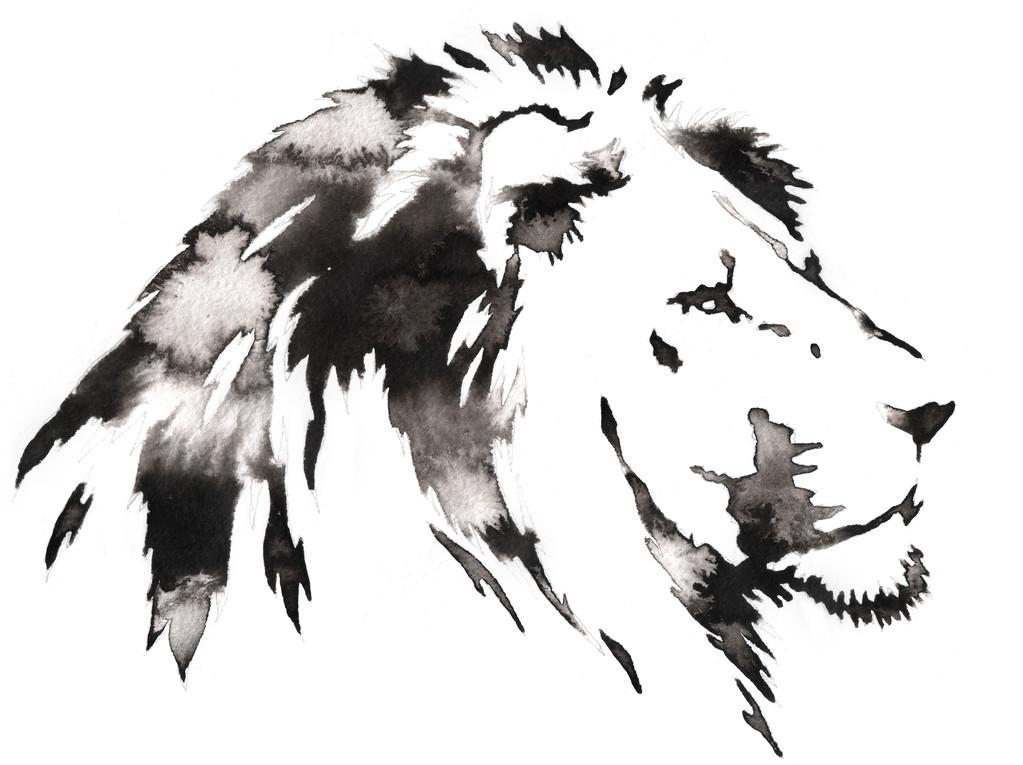
\includegraphics{lion}
    % 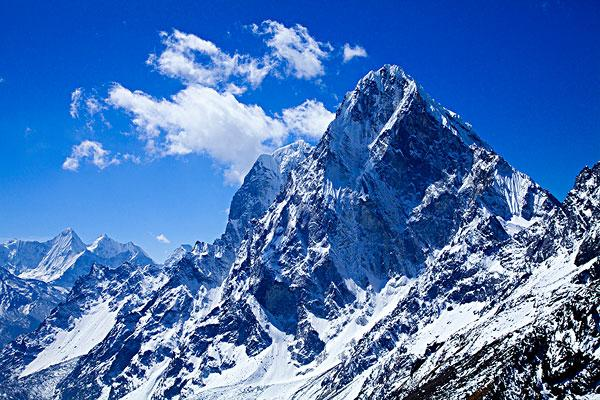
\includegraphics{mountain}
    % 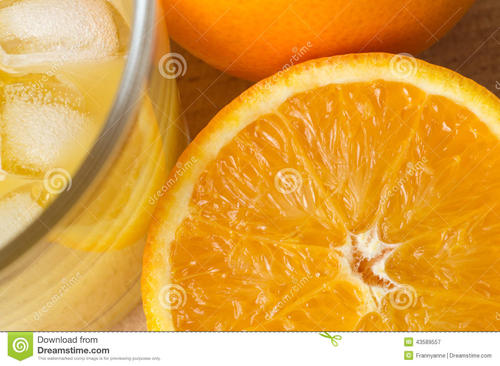
\includegraphics{orange}

    % 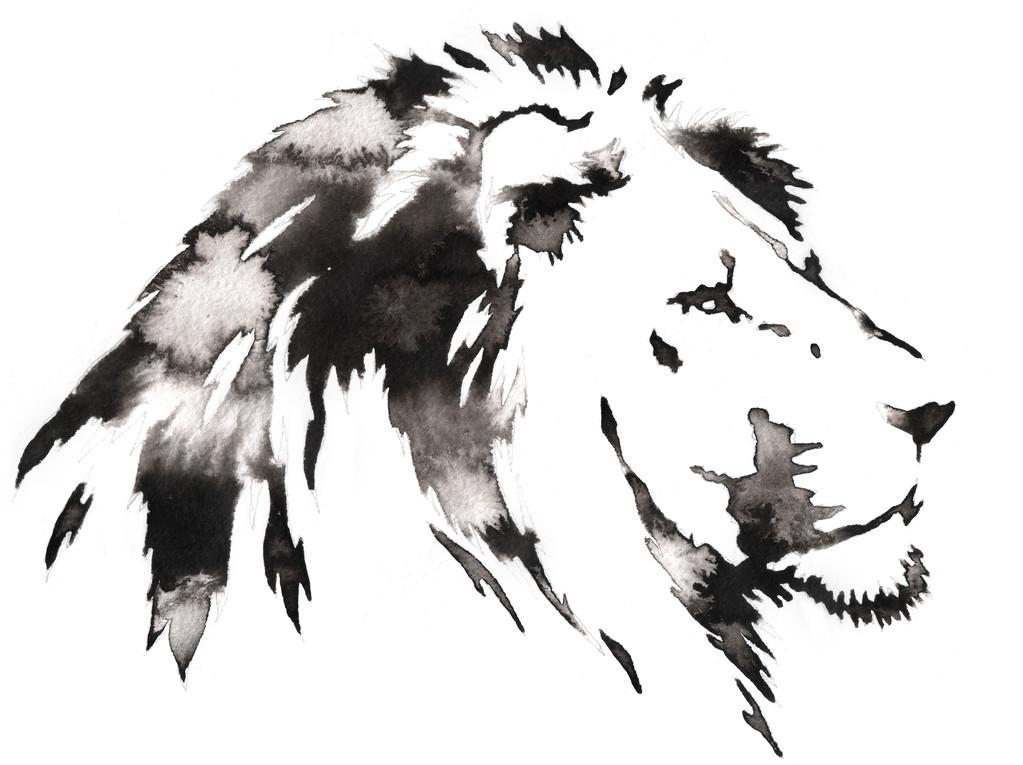
\includegraphics{lion.jpeg}
    % 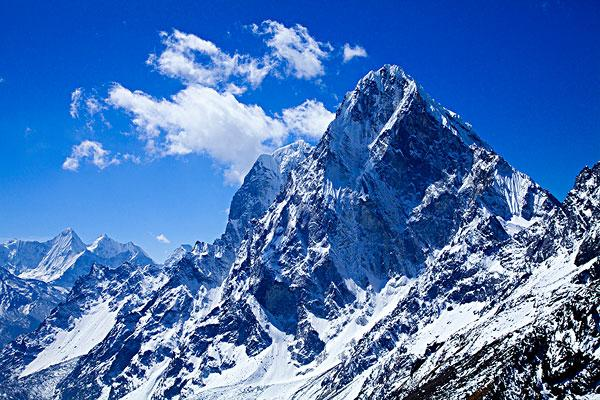
\includegraphics{mountain.jpeg}
    % 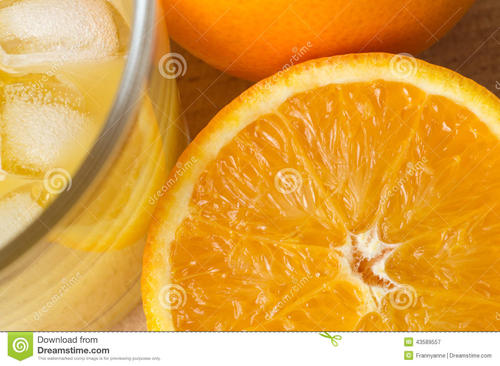
\includegraphics{orange.jpg}

    % 引入可选参数，缩放因子
    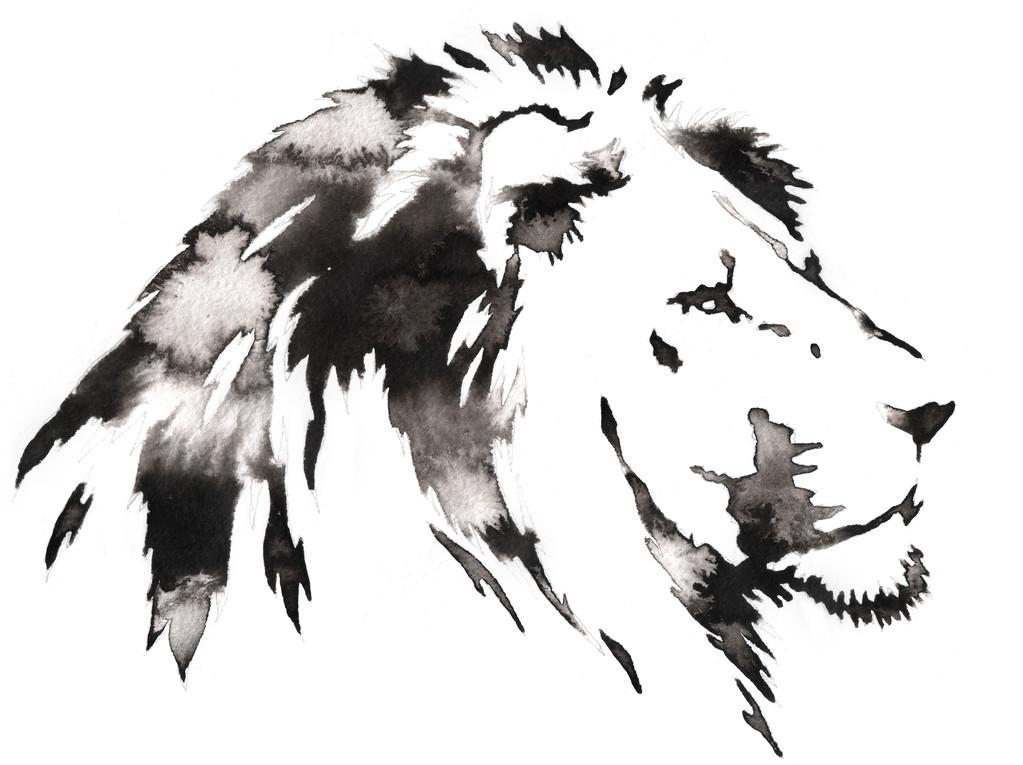
\includegraphics[scale=0.8]{lion}
    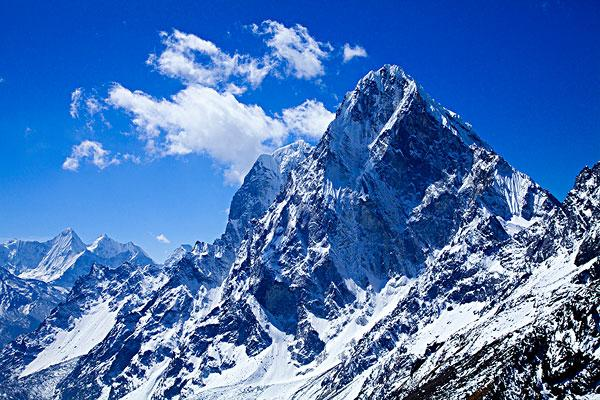
\includegraphics[scale=0.08]{mountain}
    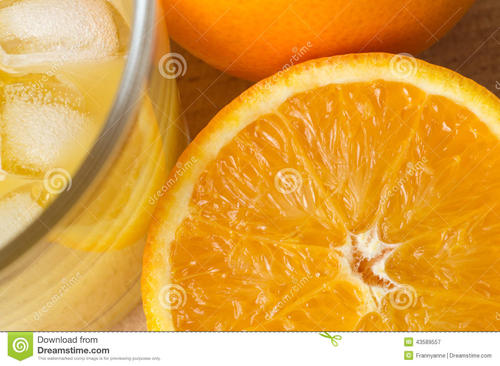
\includegraphics[scale=0.8]{orange}

    % 指定高度
    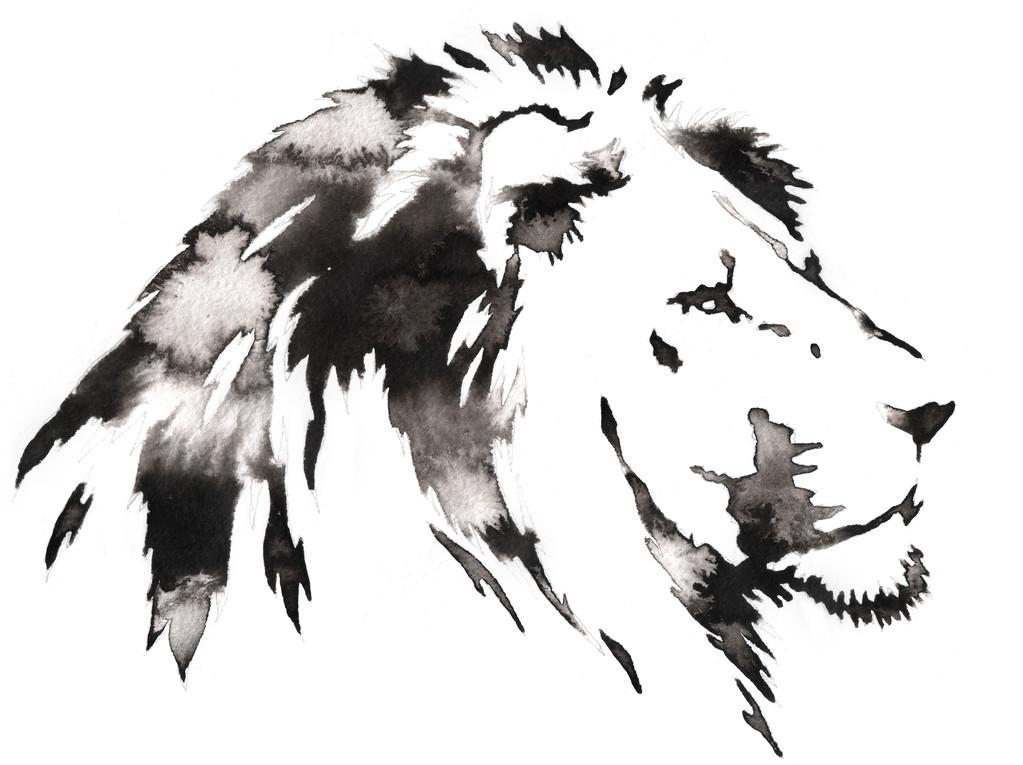
\includegraphics[height=2cm]{lion}
    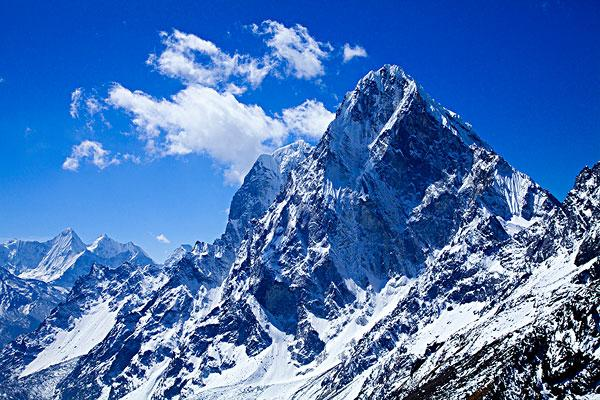
\includegraphics[height=2cm]{mountain}
    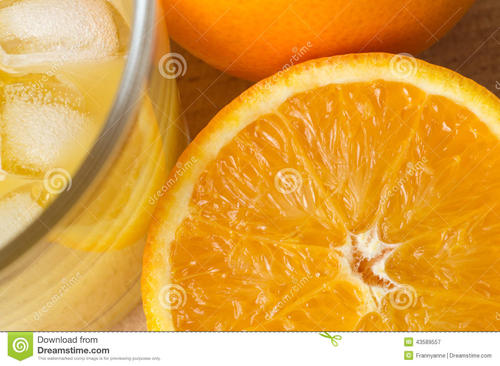
\includegraphics[height=2cm]{orange}

    % 指定宽度
    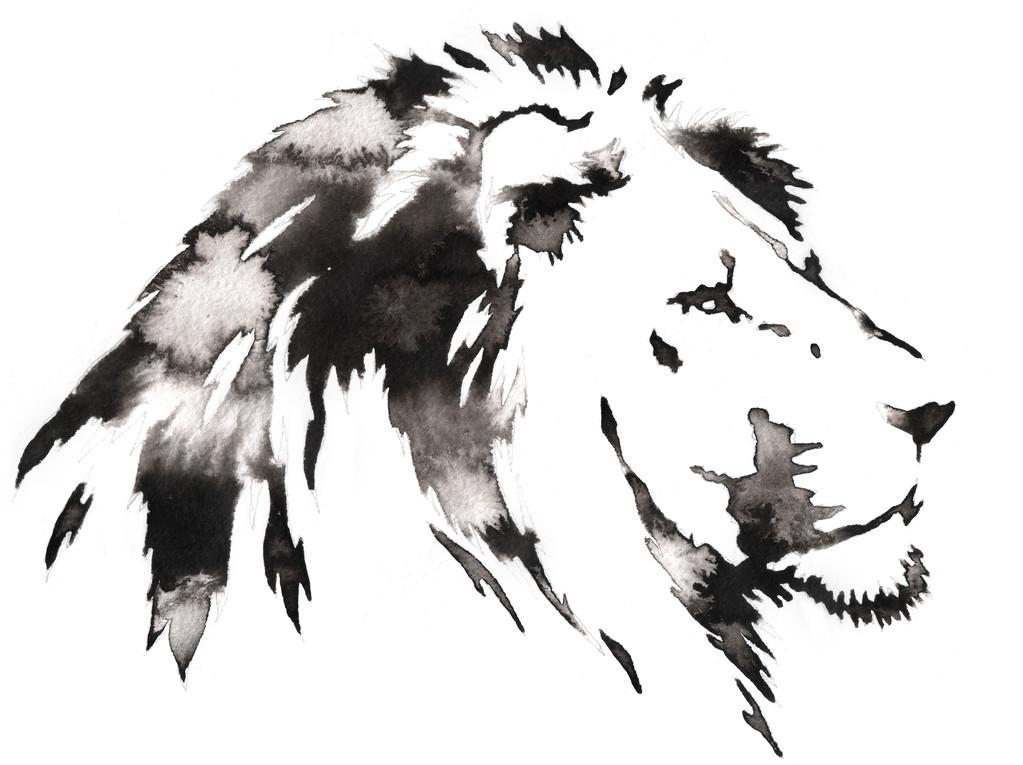
\includegraphics[width=2cm]{lion}
    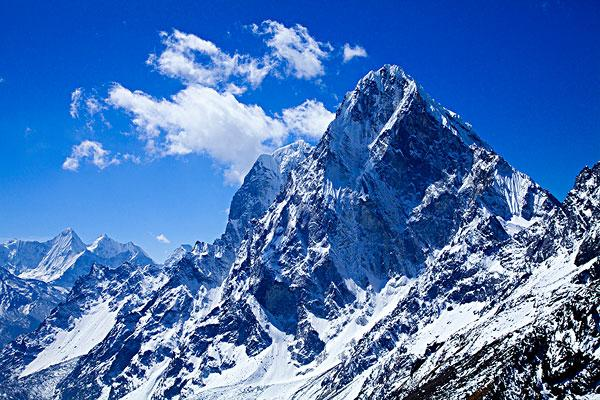
\includegraphics[width=2cm]{mountain}
    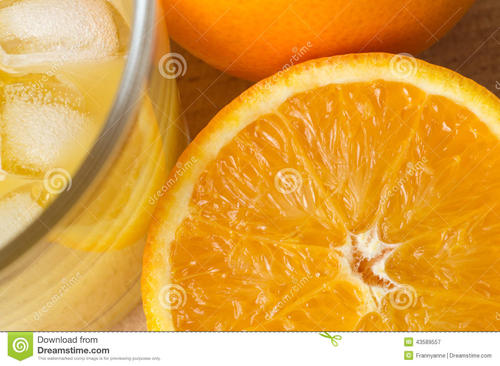
\includegraphics[width=2cm]{orange}

    % 指定相对高度
    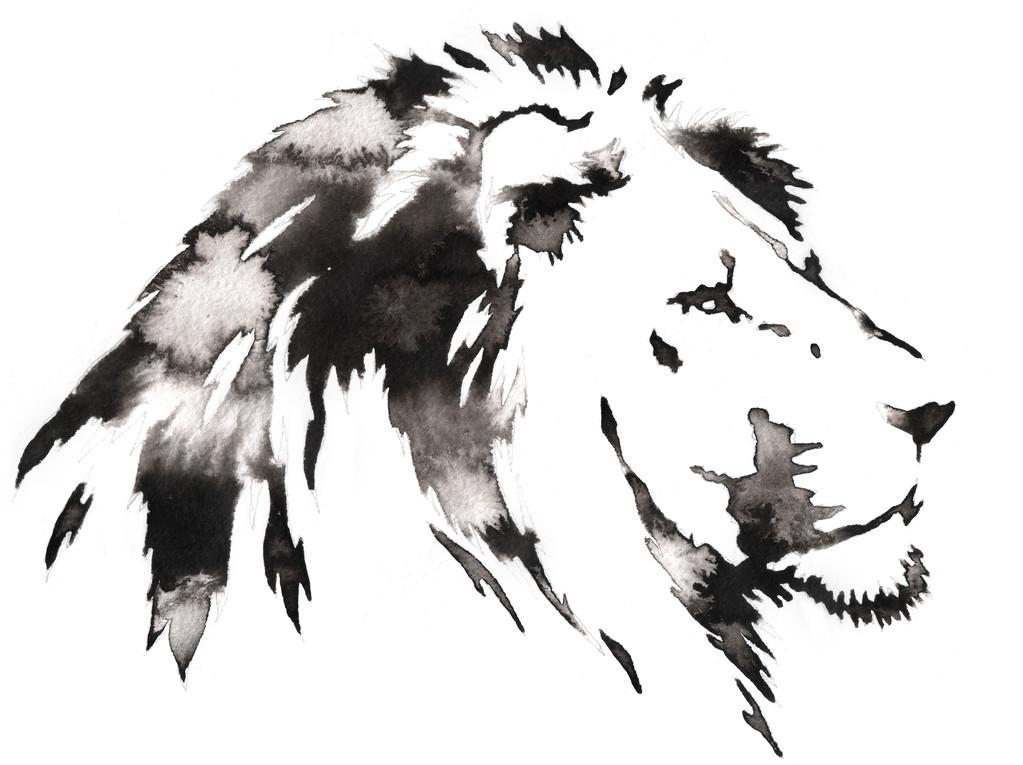
\includegraphics[height=0.1\textheight]{lion}
    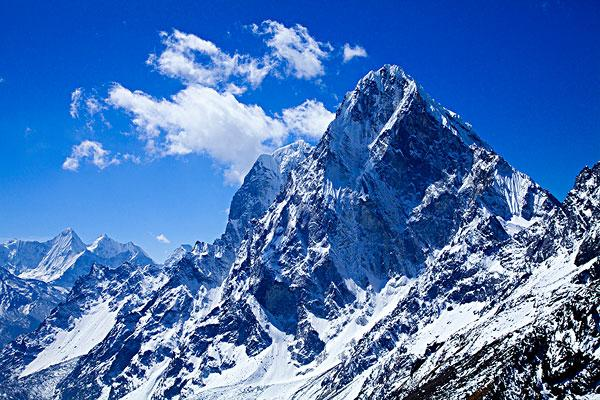
\includegraphics[height=0.1\textheight]{mountain}
    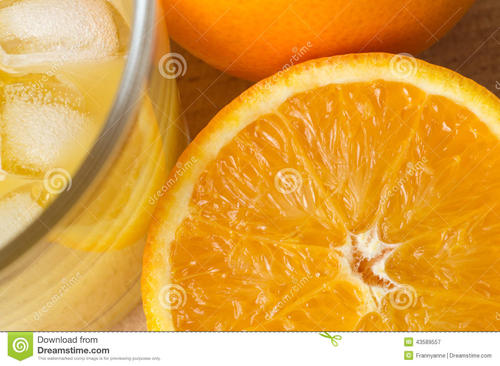
\includegraphics[height=0.1\textheight]{orange}

    % 指定相对宽度
    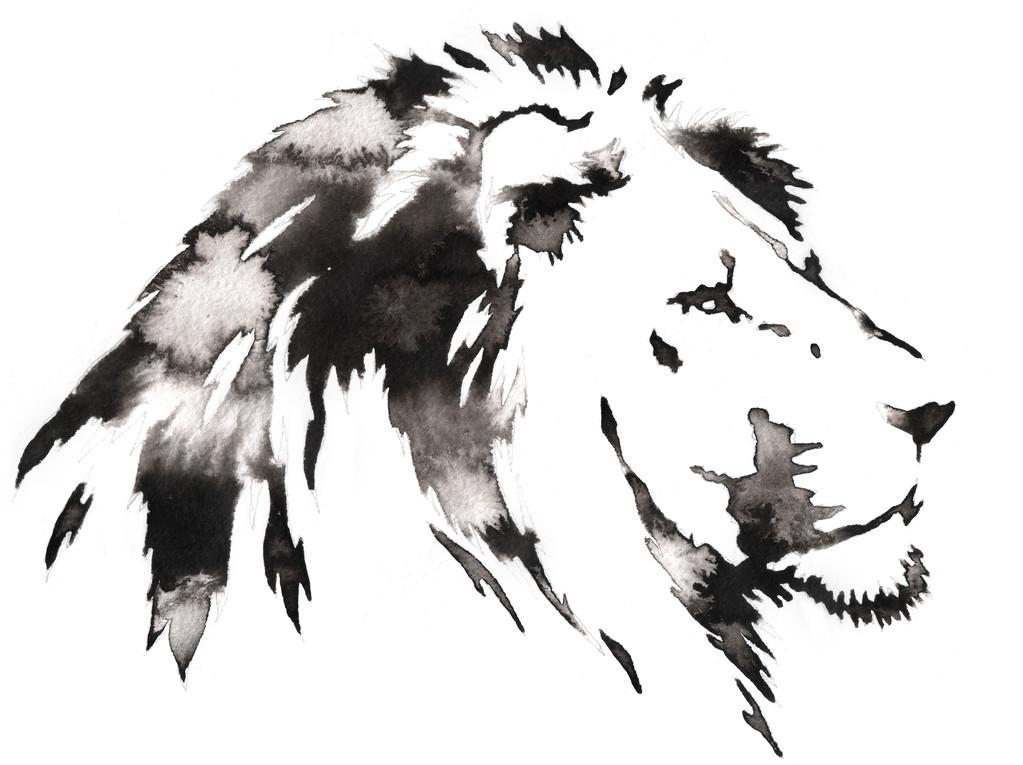
\includegraphics[height=0.2\textheight]{lion}
    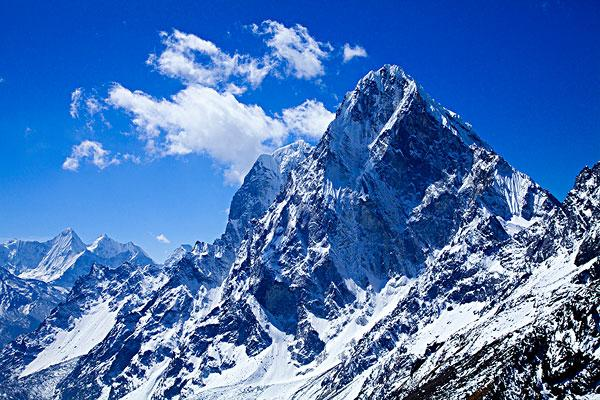
\includegraphics[height=0.2\textheight]{mountain}
    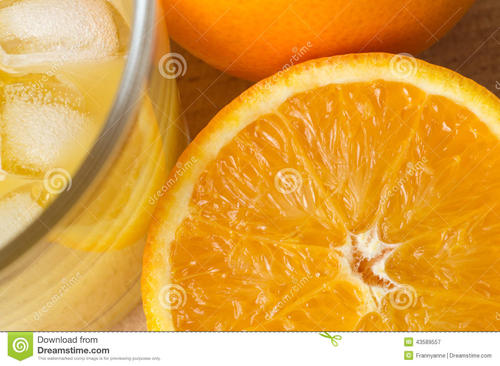
\includegraphics[height=0.2\textheight]{orange}

    % 同时指定多个参数
    % 旋转角度，不同参数使用逗号分割
    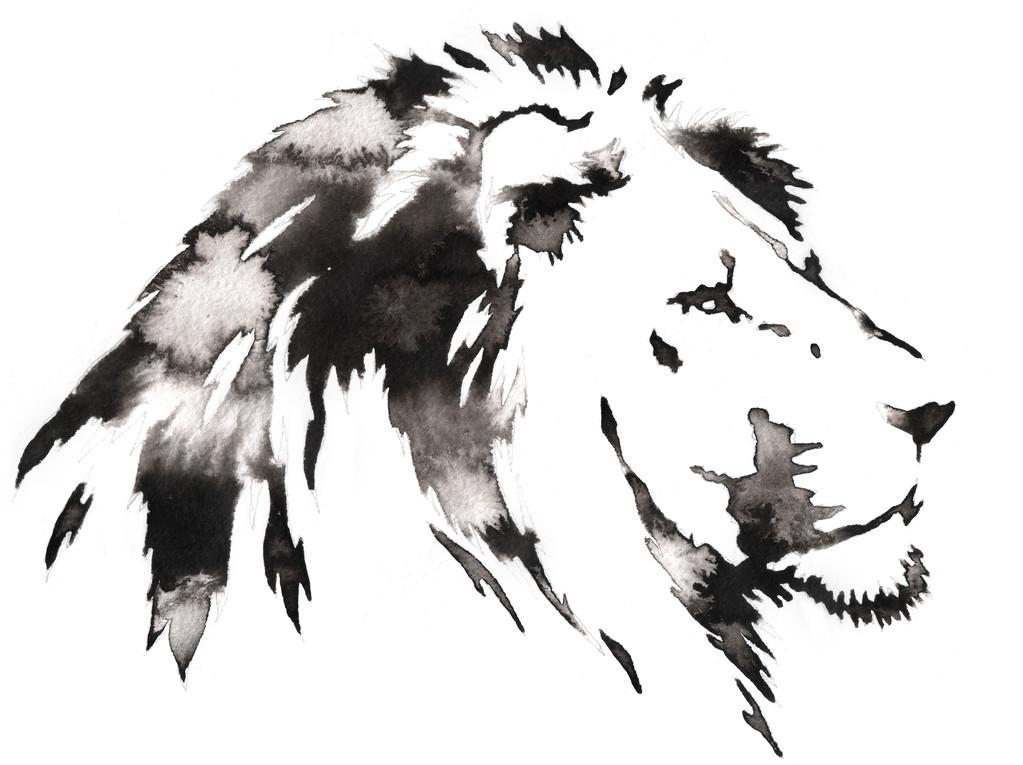
\includegraphics[angle=-45, width=0.2\textwidth]{lion}
    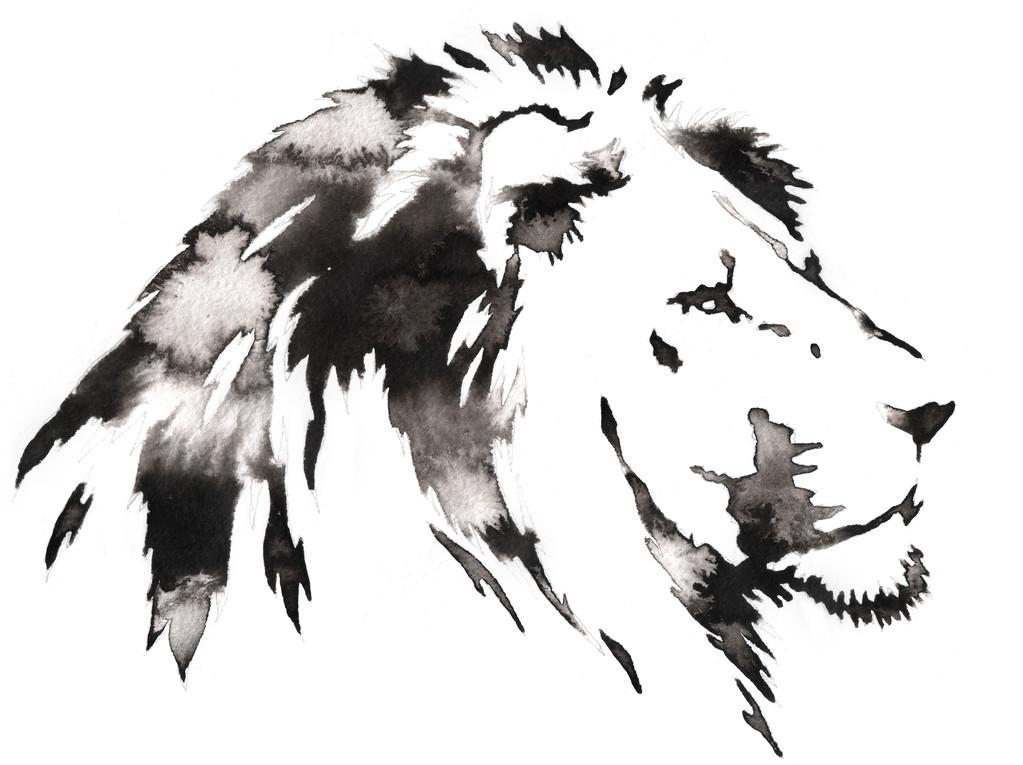
\includegraphics[width=0.2\textwidth]{lion}
    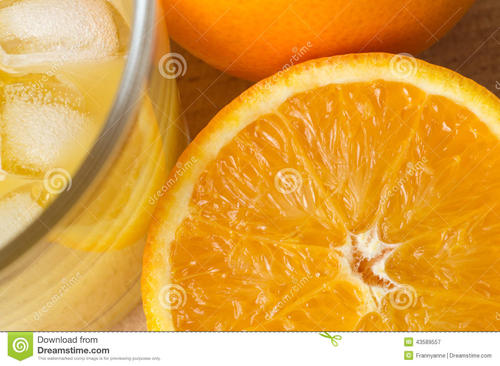
\includegraphics[angle=45, width=0.2\textwidth]{orange}
\end{document}
